


\tikzset{every picture/.style={line width=0.75pt}} %set default line width to 0.75pt        

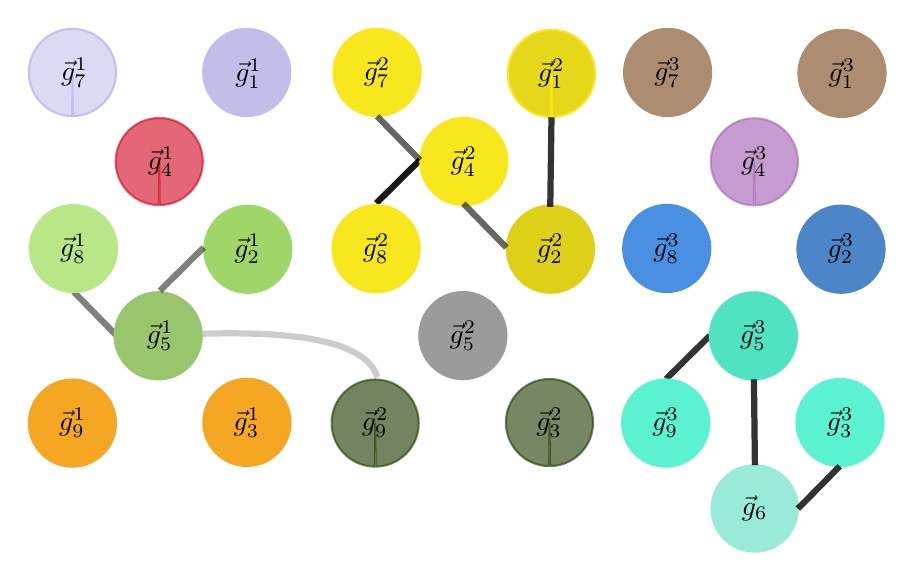
\begin{tikzpicture}[x=0.75pt,y=0.75pt,yscale=-0.7,xscale=0.7]
%uncomment if require: \path (0,1438); %set diagram left start at 0, and has height of 1438

%Straight Lines [id:da1491775175438932] 
\draw [color={rgb, 255:red, 0; green, 0; blue, 0 }  ,draw opacity=0.5 ][line width=2.25]    (71.04,641.16) -- (100.57,671.32) ;
%Shape: Pie [id:dp4189504339312904] 
\draw  [color={rgb, 255:red, 208; green, 2; blue, 27 }  ,draw opacity=0.6 ][fill={rgb, 255:red, 208; green, 2; blue, 27 }  ,fill opacity=0.6 ] (129.75,581.49) .. controls (129.75,581.49) and (129.75,581.49) .. (129.75,581.49) .. controls (113.18,581.4) and (99.82,567.89) .. (99.91,551.32) .. controls (100,534.76) and (113.5,521.4) .. (130.07,521.49) .. controls (146.64,521.58) and (160,535.08) .. (159.91,551.65) .. controls (159.82,568.04) and (146.6,581.29) .. (130.27,581.48) -- (129.91,551.49) -- cycle ;
%Shape: Pie [id:dp9353651846640743] 
\draw  [color={rgb, 255:red, 153; green, 197; blue, 108 }  ,draw opacity=1 ][fill={rgb, 255:red, 153; green, 197; blue, 108 }  ,fill opacity=1 ] (129.02,701.42) .. controls (129.02,701.42) and (129.02,701.42) .. (129.02,701.42) .. controls (112.45,701.33) and (99.09,687.83) .. (99.18,671.26) .. controls (99.27,654.69) and (112.78,641.34) .. (129.34,641.43) .. controls (145.91,641.51) and (159.27,655.02) .. (159.18,671.59) .. controls (159.09,687.98) and (145.87,701.23) .. (129.54,701.42) -- (129.18,671.42) -- cycle ;
%Shape: Pie [id:dp8579397008893295] 
\draw  [color={rgb, 255:red, 245; green, 166; blue, 35 }  ,draw opacity=1 ][fill={rgb, 255:red, 245; green, 166; blue, 35 }  ,fill opacity=1 ] (70,761.49) .. controls (70,761.49) and (70,761.49) .. (70,761.49) .. controls (53.43,761.4) and (40.07,747.89) .. (40.16,731.33) .. controls (40.25,714.76) and (53.76,701.4) .. (70.32,701.49) .. controls (86.89,701.58) and (100.25,715.08) .. (100.16,731.65) .. controls (100.07,748.04) and (86.85,761.29) .. (70.52,761.49) -- (70.16,731.49) -- cycle ;
%Shape: Pie [id:dp2502005249053001] 
\draw  [color={rgb, 255:red, 185; green, 231; blue, 136 }  ,draw opacity=1 ][fill={rgb, 255:red, 185; green, 231; blue, 136 }  ,fill opacity=1 ] (70.73,641.35) .. controls (70.73,641.35) and (70.73,641.35) .. (70.73,641.35) .. controls (54.16,641.26) and (40.8,627.76) .. (40.89,611.19) .. controls (40.98,594.62) and (54.49,581.27) .. (71.05,581.36) .. controls (87.62,581.44) and (100.98,594.95) .. (100.89,611.52) .. controls (100.8,627.91) and (87.58,641.16) .. (71.25,641.35) -- (70.89,611.35) -- cycle ;
%Shape: Circle [id:dp03941773744240962] 
\draw  [color={rgb, 255:red, 153; green, 234; blue, 216 }  ,draw opacity=1 ][fill={rgb, 255:red, 153; green, 234; blue, 216 }  ,fill opacity=1 ] (539.91,760.5) .. controls (556.34,760.59) and (569.59,773.98) .. (569.5,790.41) .. controls (569.41,806.84) and (556.02,820.09) .. (539.59,820) .. controls (523.16,819.91) and (509.91,806.52) .. (510,790.09) .. controls (510.09,773.66) and (523.48,760.41) .. (539.91,760.5) -- cycle ;
%Shape: Pie [id:dp3011559649573772] 
\draw  [color={rgb, 255:red, 245; green, 166; blue, 35 }  ,draw opacity=1 ][fill={rgb, 255:red, 245; green, 166; blue, 35 }  ,fill opacity=1 ] (190.08,761) .. controls (190.08,761) and (190.08,761) .. (190.08,761) .. controls (173.52,760.91) and (160.16,747.41) .. (160.25,730.84) .. controls (160.34,714.27) and (173.84,700.91) .. (190.41,701) .. controls (206.98,701.09) and (220.34,714.6) .. (220.25,731.16) .. controls (220.16,747.56) and (206.94,760.81) .. (190.61,761) -- (190.25,731) -- cycle ;
%Shape: Pie [id:dp8083393971230546] 
\draw  [color={rgb, 255:red, 159; green, 214; blue, 103 }  ,draw opacity=1 ][fill={rgb, 255:red, 159; green, 214; blue, 103 }  ,fill opacity=1 ] (190.71,641.87) .. controls (190.71,641.87) and (190.71,641.87) .. (190.71,641.87) .. controls (174.14,641.78) and (160.78,628.27) .. (160.87,611.71) .. controls (160.96,595.14) and (174.46,581.78) .. (191.03,581.87) .. controls (207.6,581.96) and (220.96,595.46) .. (220.87,612.03) .. controls (220.78,628.42) and (207.56,641.68) .. (191.23,641.87) -- (190.87,611.87) -- cycle ;
%Shape: Pie [id:dp14592092420046887] 
\draw  [color={rgb, 255:red, 193; green, 191; blue, 234 }  ,draw opacity=1 ][fill={rgb, 255:red, 193; green, 191; blue, 234 }  ,fill opacity=1 ][line width=0.75]  (190,520.16) .. controls (190,520.16) and (190,520.16) .. (190,520.16) .. controls (173.43,520.07) and (160.07,506.57) .. (160.16,490) .. controls (160.25,473.43) and (173.76,460.07) .. (190.32,460.16) .. controls (206.89,460.25) and (220.25,473.76) .. (220.16,490.33) .. controls (220.07,506.72) and (206.85,519.97) .. (190.52,520.16) -- (190.16,490.16) -- cycle ;
%Shape: Pie [id:dp6201888871717822] 
\draw  [color={rgb, 255:red, 195; green, 193; blue, 236 }  ,draw opacity=1 ][fill={rgb, 255:red, 195; green, 193; blue, 236 }  ,fill opacity=0.6 ] (70,520.16) .. controls (70,520.16) and (70,520.16) .. (70,520.16) .. controls (53.43,520.07) and (40.07,506.57) .. (40.16,490) .. controls (40.25,473.43) and (53.76,460.07) .. (70.32,460.16) .. controls (86.89,460.25) and (100.25,473.76) .. (100.16,490.32) .. controls (100.07,506.72) and (86.85,519.97) .. (70.52,520.16) -- (70.16,490.16) -- cycle ;
%Straight Lines [id:da1013837885900215] 
\draw [color={rgb, 255:red, 0; green, 0; blue, 0 }  ,draw opacity=0.5 ][line width=2.25]    (160.5,610.65) -- (130.34,640.48) ;
%Straight Lines [id:da23925554122471016] 
\draw [color={rgb, 255:red, 0; green, 0; blue, 0 }  ,draw opacity=0.9 ][line width=2.25]    (309.48,550.32) -- (279.32,580.16) ;
%Shape: Pie [id:dp8141174318279956] 
\draw  [color={rgb, 255:red, 248; green, 231; blue, 28 }  ,draw opacity=1 ][fill={rgb, 255:red, 248; green, 231; blue, 28 }  ,fill opacity=1 ] (339.39,581.49) .. controls (339.39,581.49) and (339.39,581.49) .. (339.39,581.49) .. controls (322.82,581.4) and (309.47,567.89) .. (309.56,551.32) .. controls (309.65,534.76) and (323.15,521.4) .. (339.72,521.49) .. controls (356.29,521.58) and (369.64,535.08) .. (369.55,551.65) .. controls (369.47,568.04) and (356.24,581.29) .. (339.92,581.48) -- (339.56,551.49) -- cycle ;
%Shape: Pie [id:dp5933933627061141] 
\draw  [color={rgb, 255:red, 155; green, 155; blue, 155 }  ,draw opacity=1 ][fill={rgb, 255:red, 155; green, 155; blue, 155 }  ,fill opacity=1 ] (338.74,701.29) .. controls (338.74,701.29) and (338.74,701.29) .. (338.74,701.29) .. controls (322.18,701.2) and (308.82,687.7) .. (308.91,671.13) .. controls (309,654.56) and (322.5,641.2) .. (339.07,641.29) .. controls (355.64,641.38) and (369,654.88) .. (368.91,671.45) .. controls (368.82,687.93) and (355.46,701.24) .. (339.01,701.29) -- (338.91,671.29) -- cycle ;
%Shape: Pie [id:dp8445434857179364] 
\draw  [color={rgb, 255:red, 34; green, 61; blue, 3 }  ,draw opacity=0.62 ][fill={rgb, 255:red, 34; green, 61; blue, 3 }  ,fill opacity=0.63 ] (278.36,761.49) .. controls (278.36,761.49) and (278.36,761.49) .. (278.36,761.49) .. controls (261.8,761.4) and (248.44,747.89) .. (248.53,731.33) .. controls (248.62,714.76) and (262.12,701.4) .. (278.69,701.49) .. controls (295.26,701.58) and (308.62,715.08) .. (308.53,731.65) .. controls (308.44,748.04) and (295.22,761.29) .. (278.89,761.49) -- (278.53,731.49) -- cycle ;
%Shape: Pie [id:dp7446890348593833] 
\draw  [color={rgb, 255:red, 248; green, 231; blue, 28 }  ,draw opacity=1 ][fill={rgb, 255:red, 248; green, 231; blue, 28 }  ,fill opacity=1 ] (279.01,641.49) .. controls (279.01,641.49) and (279.01,641.49) .. (279.01,641.49) .. controls (262.45,641.4) and (249.09,627.9) .. (249.18,611.33) .. controls (249.27,594.76) and (262.77,581.4) .. (279.34,581.49) .. controls (295.91,581.58) and (309.27,595.08) .. (309.18,611.65) .. controls (309.09,628.05) and (295.87,641.3) .. (279.54,641.49) -- (279.18,611.49) -- cycle ;
%Shape: Pie [id:dp46582212865750816] 
\draw  [color={rgb, 255:red, 34; green, 61; blue, 3 }  ,draw opacity=0.63 ][fill={rgb, 255:red, 34; green, 61; blue, 3 }  ,fill opacity=0.62 ] (398.34,761.14) .. controls (398.34,761.14) and (398.34,761.14) .. (398.34,761.14) .. controls (381.77,761.05) and (368.42,747.54) .. (368.5,730.98) .. controls (368.59,714.41) and (382.1,701.05) .. (398.67,701.14) .. controls (415.23,701.23) and (428.59,714.73) .. (428.5,731.3) .. controls (428.42,747.69) and (415.19,760.94) .. (398.87,761.14) -- (398.5,731.14) -- cycle ;
%Shape: Pie [id:dp444266981194676] 
\draw  [color={rgb, 255:red, 222; green, 207; blue, 23 }  ,draw opacity=1 ][fill={rgb, 255:red, 222; green, 207; blue, 23 }  ,fill opacity=1 ] (399.01,641.81) .. controls (399.01,641.81) and (399.01,641.81) .. (399.01,641.81) .. controls (382.45,641.72) and (369.09,628.22) .. (369.18,611.65) .. controls (369.27,595.08) and (382.77,581.72) .. (399.34,581.81) .. controls (415.91,581.9) and (429.27,595.4) .. (429.18,611.97) .. controls (429.09,628.37) and (415.87,641.62) .. (399.54,641.81) -- (399.18,611.81) -- cycle ;
%Shape: Pie [id:dp2974635390804181] 
\draw  [color={rgb, 255:red, 248; green, 231; blue, 28 }  ,draw opacity=1 ][fill={rgb, 255:red, 231; green, 215; blue, 27 }  ,fill opacity=1 ] (399.68,520.81) .. controls (399.68,520.81) and (399.68,520.81) .. (399.68,520.81) .. controls (383.11,520.72) and (369.75,507.22) .. (369.84,490.65) .. controls (369.93,474.08) and (383.43,460.72) .. (400,460.81) .. controls (416.57,460.9) and (429.93,474.41) .. (429.84,490.97) .. controls (429.75,507.37) and (416.53,520.62) .. (400.2,520.81) -- (399.84,490.81) -- cycle ;
%Shape: Pie [id:dp49974047069250127] 
\draw  [color={rgb, 255:red, 248; green, 231; blue, 28 }  ,draw opacity=1 ][fill={rgb, 255:red, 248; green, 231; blue, 28 }  ,fill opacity=1 ] (279.68,520.16) .. controls (279.68,520.16) and (279.68,520.16) .. (279.68,520.16) .. controls (263.11,520.07) and (249.75,506.57) .. (249.84,490) .. controls (249.93,473.43) and (263.43,460.07) .. (280,460.16) .. controls (296.57,460.25) and (309.93,473.76) .. (309.84,490.32) .. controls (309.75,506.72) and (296.53,519.97) .. (280.2,520.16) -- (279.84,490.16) -- cycle ;
%Straight Lines [id:da7912682226161833] 
\draw [color={rgb, 255:red, 0; green, 0; blue, 0 }  ,draw opacity=0.6 ][line width=2.25]    (279.89,520.36) -- (309.41,550.52) ;
%Straight Lines [id:da11406009939665296] 
\draw [color={rgb, 255:red, 0; green, 0; blue, 0 }  ,draw opacity=0.6 ][line width=2.25]    (339.32,580.49) -- (368.84,610.65) ;
%Straight Lines [id:da7326393920223637] 
\draw [color={rgb, 255:red, 0; green, 0; blue, 0 }  ,draw opacity=0.8 ][line width=2.25]    (399.89,521.01) -- (399.04,582.7) ;
%Straight Lines [id:da13688598404836338] 
\draw [color={rgb, 255:red, 0; green, 0; blue, 0 }  ,draw opacity=0.8 ][line width=2.25]    (508.91,671.32) -- (478.74,701.16) ;
%Shape: Pie [id:dp6886397509672018] 
\draw  [color={rgb, 255:red, 170; green, 106; blue, 183 }  ,draw opacity=0.64 ][fill={rgb, 255:red, 170; green, 106; blue, 183 }  ,fill opacity=0.67 ] (539.35,581.68) .. controls (539.35,581.68) and (539.35,581.68) .. (539.35,581.68) .. controls (522.78,581.59) and (509.42,568.09) .. (509.51,551.52) .. controls (509.6,534.95) and (523.1,521.59) .. (539.67,521.68) .. controls (556.24,521.77) and (569.6,535.27) .. (569.51,551.84) .. controls (569.42,568.24) and (556.2,581.49) .. (539.87,581.68) -- (539.51,551.68) -- cycle ;
%Shape: Pie [id:dp2803763676379287] 
\draw  [color={rgb, 255:red, 80; green, 227; blue, 194 }  ,draw opacity=1 ][fill={rgb, 255:red, 80; green, 227; blue, 194 }  ,fill opacity=1 ] (538.7,701.48) .. controls (538.7,701.48) and (538.7,701.48) .. (538.7,701.48) .. controls (522.13,701.39) and (508.77,687.89) .. (508.86,671.32) .. controls (508.95,654.75) and (522.45,641.39) .. (539.02,641.48) .. controls (555.59,641.57) and (568.95,655.08) .. (568.86,671.65) .. controls (568.77,688.04) and (555.55,701.29) .. (539.22,701.48) -- (538.86,671.48) -- cycle ;
%Shape: Pie [id:dp829468873726058] 
\draw  [color={rgb, 255:red, 90; green, 242; blue, 208 }  ,draw opacity=1 ][fill={rgb, 255:red, 90; green, 242; blue, 208 }  ,fill opacity=1 ] (478.34,761.49) .. controls (478.34,761.49) and (478.34,761.49) .. (478.34,761.49) .. controls (461.77,761.4) and (448.41,747.89) .. (448.5,731.33) .. controls (448.59,714.76) and (462.09,701.4) .. (478.66,701.49) .. controls (495.23,701.58) and (508.59,715.08) .. (508.5,731.65) .. controls (508.41,748.04) and (495.19,761.29) .. (478.86,761.49) -- (478.5,731.49) -- cycle ;
%Shape: Pie [id:dp40484909174697115] 
\draw  [color={rgb, 255:red, 74; green, 144; blue, 226 }  ,draw opacity=1 ][fill={rgb, 255:red, 74; green, 144; blue, 226 }  ,fill opacity=1 ] (479.07,641.3) .. controls (479.07,641.3) and (479.07,641.3) .. (479.07,641.3) .. controls (462.5,641.21) and (449.14,627.7) .. (449.23,611.13) .. controls (449.32,594.57) and (462.82,581.21) .. (479.39,581.3) .. controls (495.96,581.39) and (509.32,594.89) .. (509.23,611.46) .. controls (509.14,627.85) and (495.92,641.1) .. (479.59,641.29) -- (479.23,611.3) -- cycle ;
%Shape: Pie [id:dp9825838812327261] 
\draw  [color={rgb, 255:red, 90; green, 242; blue, 208 }  ,draw opacity=1 ][fill={rgb, 255:red, 90; green, 242; blue, 208 }  ,fill opacity=1 ] (598.34,761.14) .. controls (598.34,761.14) and (598.34,761.14) .. (598.34,761.14) .. controls (581.77,761.05) and (568.42,747.54) .. (568.5,730.98) .. controls (568.59,714.41) and (582.1,701.05) .. (598.67,701.14) .. controls (615.23,701.23) and (628.59,714.73) .. (628.5,731.3) .. controls (628.42,747.69) and (615.19,760.94) .. (598.87,761.14) -- (598.5,731.14) -- cycle ;
%Shape: Pie [id:dp1374121111076505] 
\draw  [color={rgb, 255:red, 76; green, 133; blue, 200 }  ,draw opacity=1 ][fill={rgb, 255:red, 76; green, 133; blue, 200 }  ,fill opacity=1 ] (598.99,641.81) .. controls (598.99,641.81) and (598.99,641.81) .. (598.99,641.81) .. controls (582.42,641.72) and (569.06,628.22) .. (569.15,611.65) .. controls (569.24,595.08) and (582.74,581.72) .. (599.31,581.81) .. controls (615.88,581.9) and (629.24,595.4) .. (629.15,611.97) .. controls (629.06,628.37) and (615.84,641.62) .. (599.51,641.81) -- (599.15,611.81) -- cycle ;
%Shape: Pie [id:dp2605597403441984] 
\draw  [color={rgb, 255:red, 173; green, 141; blue, 113 }  ,draw opacity=1 ][fill={rgb, 255:red, 173; green, 141; blue, 113 }  ,fill opacity=1 ] (599.68,520.81) .. controls (599.68,520.81) and (599.68,520.81) .. (599.68,520.81) .. controls (583.11,520.72) and (569.75,507.22) .. (569.84,490.65) .. controls (569.93,474.08) and (583.43,460.72) .. (600,460.81) .. controls (616.57,460.9) and (629.93,474.41) .. (629.84,490.97) .. controls (629.75,507.37) and (616.53,520.62) .. (600.2,520.81) -- (599.84,490.81) -- cycle ;
%Shape: Pie [id:dp26916903671793757] 
\draw  [color={rgb, 255:red, 173; green, 141; blue, 113 }  ,draw opacity=1 ][fill={rgb, 255:red, 173; green, 141; blue, 113 }  ,fill opacity=1 ] (479.68,520.16) .. controls (479.68,520.16) and (479.68,520.16) .. (479.68,520.16) .. controls (463.11,520.07) and (449.75,506.57) .. (449.84,490) .. controls (449.93,473.43) and (463.43,460.07) .. (480,460.16) .. controls (496.57,460.25) and (509.93,473.76) .. (509.84,490.32) .. controls (509.75,506.72) and (496.53,519.97) .. (480.2,520.16) -- (479.84,490.16) -- cycle ;
%Straight Lines [id:da5982033983596651] 
\draw [color={rgb, 255:red, 0; green, 0; blue, 0 }  ,draw opacity=0.8 ][line width=2.25]    (569.5,790.41) -- (598.34,761.14) ;
%Straight Lines [id:da16999475415741472] 
\draw [color={rgb, 255:red, 0; green, 0; blue, 0 }  ,draw opacity=0.8 ][line width=2.25]    (539.22,701.48) -- (539.91,760.5) ;
%Curve Lines [id:da9163583164432756] 
\draw [color={rgb, 255:red, 0; green, 0; blue, 0 }  ,draw opacity=0.2 ][line width=2.25]    (160,670) .. controls (216.8,668.4) and (272.04,673.12) .. (280,700) ;


\draw (190.25,731) node [align=left] {$\vec g_3^1$};

\draw (71.5,490.22) node [align=left] {$\vec g_{7}^1$};
% Text Node
\draw (130.57,671.29) node [align=left] {$\vec g_{5}^1$};
% Text Node
\draw (70.89,611.35) node [align=left] {$\vec g_{8}^1$};
% Text Node
\draw (539.75,790.25) node [align=left] {$\vec g_{6}$};
% Text Node
\draw (131.22,551.49) node [align=left] {$\vec g_{4}^1$};
% Text Node
\draw (190.84,611.81) node [align=left] {$\vec g_{2}^1$};
% Text Node
\draw (191.42,491.01) node [align=left] {$\vec g_{1}^1$};
% Text Node
\draw (70.19,731.49) node [align=left] {$\vec g_{9}^1$};
% Text Node
\draw (398.58,731) node  [align=left] {$\vec g_{3}^2$};
% Text Node
\draw (279.84,490.22) node [align=left] {$\vec g_{7}^2$};
% Text Node
\draw (338.91,671.29) node   [align=left] {$\vec g_{5}^2$};
% Text Node
\draw (279.23,611.35) node  [align=left] {$\vec g_{8}^2$};
% Text Node
\draw (339.56,551.49) node  [align=left] {$\vec g_{4}^2$};
% Text Node
\draw (399.18,611.81) node  [align=left] {$\vec g_{2}^2$};
% Text Node
\draw (399.76,491.01) node  [align=left] {$\vec g_{1}^2$};
% Text Node
\draw (278.53,731.49) node [align=left] {$\vec g_{9}^2$};
% Text Node
\draw (598.58,731) node  [align=left] {$\vec g_{3}^3$};
% Text Node
\draw (479.84,490.22) node  [align=left] {$\vec g_{7}^3$};
% Text Node
\draw (538.91,671.29) node [align=left] {$\vec g_{5}^3$};
% Text Node
\draw (479.23,611.35) node [align=left] {$\vec g_{8}^3$};
% Text Node
\draw (539.56,551.49) node [align=left] {$\vec g_{4}^3$};
% Text Node
\draw (599.18,611.81) node [align=left] {$\vec g_{2}^3$};
% Text Node
\draw (599.76,491.01) node [align=left] {$\vec g_{1}^3$};
% Text Node
\draw (478.53,731.49) node [align=left] {$\vec g_{9}^3$};


\end{tikzpicture}